\documentclass[runningheads]{llncs}
\usepackage[T1]{fontenc}
\usepackage{graphicx}
\usepackage{subcaption}
\usepackage{enumitem}

% \usepackage{changes}  % Using the changes package
% \usepackage[final]{changes} % Disable revisions, output the final revised version
% \usepackage[commandnameprefix=always, defaultcolor=red]{changes}  % Using the changes package
% \definechangesauthor[name={zheliku}, color=blue]{zheliku} % Revision author

\bibliographystyle{splncs04}

\AtBeginDocument{%
  \providecommand\BibTeX{{%
  Bib\TeX}}}

\begin{document}
\title{VRTI: Gesture Interaction Supporting Passive Haptics and Haptic Retargeting to Enhance Immersive Learning Experiences}
% \author{Hailin Ji\inst{1} \and
% % \orcidID{0009-0002-3512-6730}
% Yihang Li\inst{1} \and
% Yiran Zhang\inst{1} \and
% Hongwen Zhang\inst{1} \and
% Xiaoyan Hu\inst{1} \and
% Yanhong Luo\inst{2}}
% \authorrunning{H. Ji et al.}
% \institute{Beijing Normal University, Beijing, China \and
% Northwest Minzu University, Beijing, China}
\author{Anonymous Authors}

\maketitle

\begin{abstract}
The use of Gesture Interaction (GI) in immersive learning environments can provide an intuitive learning experience, but the lack of force and haptic feedback significantly weakens its sense of immersion. Traditional active haptic solutions limit the interaction flexibility of GI, while passive haptic solutions struggle to meet dynamic interaction needs. To address these issues, this paper proposes the Virtual-Reality Twin Interaction (VRTI) framework, which adopts Dynamic Passive Haptic Feedback (DPHF) and Haptic Retargeting (HR) technologies to provide dynamic passive haptic feedback for gesture interaction. Meanwhile, based on VRTI, a Virtual-Reality Twin (VRT) prototype supporting three basic operations: grasping, pressing, and pinching is implemented and applied in an immersive learning environment. Finally, user studies show that compared with the GI group, the VRTI group significantly improves users' learning motivation (p<0.001) and sense of presence (p<0.001).

\keywords{Virtual Reality \and Passive Haptic Feedback \and Haptic Retargeting \and Gesture Interaction \and Immersive Learning}
\end{abstract}

\section{Introduction}
Gesture Interaction (GI), as one of the most natural interaction methods in Virtual Reality (VR), has shown significant advantages in immersive learning environments \cite{fang2024interactive,amaral2024interactive}. However, the current visually dominated interaction paradigm has a key limitation - the lack of real haptic feedback. This deficiency seriously restricts the sense of immersion and interaction effectiveness of virtual reality in educational applications.

Currently, mainstream haptic feedback solutions can be divided into two categories: active and passive. Active haptics use actuators to actively apply forces to users (such as force feedback gloves), providing a dynamic range of haptic feedback. However, their bulky equipment and limited interaction characteristics restrict their popularization in educational scenarios \cite{bonfert2023challenges,shigeyama2019transcalibur}. Passive haptics place physical objects (also known as proxies or props) at the location of virtual objects, allowing users to touch the physical surface to obtain haptics \cite{hinckley1994passive}. However, existing passive haptic methods mostly rely on static props \cite{strandholt2020knock,fang2023vr,rettinger2023touching}, which cannot adapt to the dynamic interaction needs common in immersive learning environments.

In recent years, Dynamic Passive Haptic Feedback (DPHF) technology has provided new possibilities to solve this dilemma \cite{zenner2017shifty}. It uses actuators to change passive haptic properties (such as size, shape, weight, weight distribution, texture, temperature, position, orientation, function, etc.) to adapt to users' interaction needs, thereby providing more natural haptic feedback. Compared with traditional passive haptic proxies, DPHF proxies adjust their passive haptic responses according to the virtual objects they represent, thereby improving the haptic realism of VR interactions. André Zenner et al. first combined DPHF with Haptic Retargeting (HR) and found that the combination of the two can make users less aware of haptic misalignment, proving that the combination of DPHF technology and HR has significant application potential \cite{zenner2021combining}, but related research is still in its infancy.

To sum up, the main contributions of this study are as follows:

\begin{enumerate}[label={\arabic*)}]
  \item Proposing Virtual-Reality Twin Interaction (VRTI), a DPHF/HR scheme integrating gesture interaction, supporting multiple gesture interaction operations and dynamic haptic feedback.
  \item Implementing three types of VRT (pull rod, button, and knob) based on VRTI, which support grasping, pressing, and pinching operations respectively, and applying them to the immersive learning environment of high school momentum conservation law.
  \item Proving the effectiveness of VRTI through user research (N=64): compared with traditional gesture interaction (GI), VRTI significantly improves users' learning motivation (p<0.001) and sense of immersion (p<0.001).
\end{enumerate}

\section{Related Work}
\subsection{Gesture Interaction}
Gesture interaction, as an important research direction in the field of human-computer interaction, realizes intention expression and operation control by recognizing upper limb postures or movements \cite{yang2019gesture}, and has shown significant advantages in immersive environments such as virtual reality and augmented reality (AR) \cite{10574578}. Relevant studies have shown that compared with other parts of the body, the dexterity and operability of hands in transmitting information and performing tasks make them ideal tools for human-computer interaction \cite{karam2006framework}. The core value of gesture interaction is reflected in three aspects \cite{mitra2007gesture,10580881,app14114935}: the first is dexterity, users can complete interactions through hand movements without additional hardware, reducing operation friction; the second is immediacy, which can be deeply integrated with VR devices to achieve seamless recognition; the last is naturalness and intuitiveness, enhancing the interaction experience by simulating real hand movements (such as grasping, rotating).

Gesture design needs to follow principles such as user orientation, cultural adaptation, system consistency, and real-time feedback \cite{lou2018analysis}. For example, the 11 basic gesture sets (such as pinching, grasping, rotating) proposed by Wu Y et al. clarify the mapping relationship of common operation tasks \cite{wu2024empirical}, while Herbert O M et al. distinguish information transmission and complex action control through static/dynamic classification \cite{herbert2024static}. In the field of virtual reality, gesture interaction has been widely used in immersive game control and education and training scenarios \cite{10574578,lu2024chemical}, significantly improving user immersion and interaction efficiency \cite{10580881}, and helping to enhance learning motivation and knowledge mastery \cite{lu2024chemical}.

However, gesture interaction still has the following limitations \cite{herbert2024static,app14114935}: first, sensor limitations, occlusion and lighting changes can lead to tracking failure; second, intention ambiguity, the randomness of gestures in natural dialogue makes it difficult to accurately parse user purposes; finally, the lack of haptic feedback, the lack of user sensory stimulation, leading to reduced immersion when operating virtual objects.

\subsection{Passive Haptics}
Haptic technologies in virtual reality can be divided into two categories: active haptics and passive haptics. Active haptic technology uses mechanical and electronic control devices to generate controllable physical forces through motor, hydraulic or pneumatic systems, acting on the user's hands or body, thereby simulating force and haptic feedback in the real environment \cite{vaghela2021active}. Passive haptics is a technology that reuses physical props or environments to create haptic sensations in VR and AR, first proposed by Insko et al. \cite{insko2001passive}. It uses physical proxies to transmit feedback through shape, thereby endowing virtual objects with physical dimensions. Passive haptic technology enables users to control and manipulate 3D virtual models more flexibly and accurately without special haptic equipment, thus having high adaptability and deployability \cite{henderson2008opportunistic,shapira2016tactilevr,10.1145/3313831.3376313}.

The implementation of passive haptic feedback mainly faces the following two challenges. First, how to design and manufacture suitable physical proxies so that they are sufficiently similar in haptic characteristics. Second, how to achieve precise alignment with physical proxies in the virtual environment to achieve seamless interaction \cite{zenner2021combining}. In addition, passive haptic technology usually requires users to have direct contact with physical proxies, which may limit its use in certain application scenarios. In recent years, Dynamic Passive Haptic Feedback (DPHF) technology has become an important development direction in the field of passive haptics. This type of technology combines the characteristics of active haptics and passive haptics, usually equipping physical proxies with real-time sensing and actuators (such as motors, actuators), which automatically adjust the state of physical proxies during user interaction to achieve high-fidelity synchronization between virtual and reality. DPHF integrates deformable, movable or adjustable physical proxies, so that their haptic properties (such as position, shape, resistance, etc.) can dynamically change according to the needs of the virtual environment, enhancing users' sense of immersion and interaction interest \cite{zenner2017shifty}.

\subsection{Haptic Retargeting}
Passive haptic technology requires physical proxies to synchronously correspond to virtual objects, which has high requirements for the physical scene. To solve this problem, Haptic Retargeting (HR) technology is proposed. HR maps multiple virtual objects to physical proxies by deceiving human perception, thereby providing users with passive haptic feedback. Previous haptic retargeting methods can be divided into two categories. The first type of method changes the virtual environment to match the geometry of the physical proxy \cite{zenner2017shifty,10.1145/2858036.2858226}. The second type of method achieves retargeting by changing the user's hand position \cite{zenner2019estimating,hartfill2021analysis}, also known as Hand Retargeting \cite{zenner2021hart}.

The core challenge of HR technology is how to realize the mapping between virtual and physical objects without being noticed by users. Current studies have shown that the maximum virtual hand deviation that users can tolerate is 40° \cite{10.1145/3025453.3025753}, and the perception threshold for hand rotation deviation is about 9° \cite{zenner2019estimating}. To maximize the possibility of users not perceiving haptic retargeting, Zenner et al. proposed combining DPHF with HR, which can make users ignore larger spatial misalignment between proxies and virtual counterparts. In addition, more efficient and comfortable haptic retargeting methods are constantly being proposed. Sun et al. proposed a haptic retargeting method based on reset points, which dynamically adjusts the position of reset points during user's hand movement, reduces users' perception of hand position changes, and significantly improves retargeting efficiency and comfort \cite{10816517}.

\section{VRTI}
We propose the VRTI interaction framework, whose core VRT consists of a pair of real interaction objects in the physical world (Real Interaction Object, RIO) and their corresponding virtual interaction objects in the virtual environment (Virtual Interaction Object, VIO), as shown in Figure \ref{fig:VRTI}. RIO adopts DPHF technology, integrating sensors and actuators to provide users with dynamic passive haptic feedback; VIO is synchronized with RIO in real-time in the virtual scene, and integrates gesture tracking and HR technology to support multiple gesture interactions and provide visual feedback synchronized with haptics.

\begin{figure*}[t]
  \centering
  \includegraphics[width=1\textwidth]{image/VRTI.pdf}
  \caption{VRTI interaction framework}
  \label{fig:VRTI}
\end{figure*}

\subsection{Proof of Concept}
For the three gestures of grasping, pressing, and pinching, we designed the following three types of VRT for verification:

\begin{enumerate}[label={\arabic*)}]
  \item \texttt{Puller} provides grasping gesture interaction, feeding back tension proportional to the pulling distance;
  \item \texttt{Button} provides pressing gesture interaction, feeding back elastic force proportional to the pressing distance;
  \item \texttt{Knob} provides pinching gesture interaction, feeding back the haptics of pinching small objects.
\end{enumerate}

Figure \ref{fig:interaction-flow} shows the interaction flow of the three. In the grasping interaction, the user holds the slider, pulls the spring backward to a specific distance to trigger the pull rod, and releases the slider to make the spring rebound to complete the interaction; in the pressing interaction, the user places their hand above the switch, presses to a specific distance to activate the button, and lifts their hand to complete the interaction; in the pinching interaction, the user pinches the head of the handle with their fingers, rotates around the central axis to adjust the angle, and releases their hand to complete the interaction.

\begin{figure*}[t]
  \centering
  \includegraphics[width=1\textwidth]{image/Interaction-Flow.pdf}
  \caption{Interaction flow of three types of VRT}
  \label{fig:interaction-flow}
\end{figure*}

\subsection{DPHF Implementation}
The data communication between VIO and RIO of VRT is realized through real-time sensing technology. Sensors are used to collect the physical properties of RIO, and the data is transmitted to Unity by Arduino after Kalman filtering. Figure \ref{fig:structural-diagram} shows the structural design of each component. Both RIO and VIO of the three are derived from the same 3D model: RIO is obtained through 3D printing, and VIO is created by importing the model into Unity. Since the user's visual feedback is directly provided by VIO, VIO is colored and rendered in the virtual environment, while RIO remains uncolored.

\begin{figure*}[t]
  \centering
  \includegraphics[width=1\textwidth]{image/Structural-Diagram.pdf}
  \caption{Structural diagram of three types of VRT}
  \label{fig:structural-diagram}
\end{figure*}

\subsubsection{Sensors and Actuators}
The sensors and actuators equipped with the three types of VRT are introduced as follows:

\begin{enumerate}[label={\arabic*)}]
  \item \texttt{Puller} For grasping gestures, a combination of a tension sensor and a spring is used. The tension sensor is installed at the connection between the spring and the block to detect the tension applied by the user in real-time. Its acquisition frequency is 50Hz, the tension measurement range is 0N to 20N, and the accuracy is ±0.1N. The spring acts as a simple actuator, restoring the object to its original position after each pull.
  \item \texttt{Button} For pressing gestures, a combination of a membrane pressure sensor and a spring is used. The membrane pressure sensor is placed at the bottom of the spring. When the user presses the button, the user's pressure is collected through the spring's elastic force. The sensor's acquisition frequency is 100Hz, the collected pressure range is 0N\(\sim\)10N, and the resolution is 0.01N. The spring also acts as a simple actuator, restoring the object to its original position after each press.
  \item \texttt{Knob} For pinching gestures, an angle sensor is used to detect the rotation angle of the knob in real-time. The angle sensor is installed at the center of the rotating shaft, capturing the rotation state of the knob at a sampling frequency of 50Hz, with an angle measurement accuracy of ±0.5 degrees.
\end{enumerate}

\subsubsection{Data Communication}
A robust communication architecture ensures low-latency data transmission of RIO. Arduino UNO is used as an interface to collect raw sensor data, and after input noise reduction, normalization, and state prediction processes, data signals are identified.

\begin{enumerate}[label={\arabic*)}]
  \item \texttt{Input Noise Reduction} Kalman filtering is applied to the raw data \(x\), and the state is estimated by optimally combining prediction and noisy measurements.
  \item \texttt{Normalization} The raw data \(x\) is normalized to a unified range [0,1] to get \(\bar{x}=(x-x_{\min})/(x_{\max}-x_{\min})\). The lower limit \(x_{\min}\) usually corresponds to the initial/static state of RIO, and the upper limit \(x_{\max}\) captures the expected maximum value through repeated user tests.
  \item \texttt{Smoothing Processing} An empirical threshold \(\varepsilon\) is used to detect state changes. When \(\bar{x}>\varepsilon\), it indicates that data input starts, and \(\Delta\bar{x}>\varepsilon\) indicates a state switch.
\end{enumerate}
\subsection{HR Implementation}
By spatially corresponding VIO and RIO, the synchronization of haptic feedback between virtual and real is ensured. Our haptic retargeting achieves seamless integration of vision and haptics through gesture recognition and a predefined interaction library.

\subsubsection{Spatial Calibration}
Ensuring the spatial correspondence between VIO and RIO is crucial for providing truly synchronized visual and haptic feedback, which can maximize the immersive experience of users. RIO is installed on a flat panel in a fixed spatial relationship to establish a physical reference frame. VIO is constructed by defining a scale between virtual units (Unity units) and real units (meters) to match the relative position and orientation of RIO in the physical reference frame.

\subsubsection{Haptic Retargeting}
The hand estimation error generated by gesture tracking technology leads to visual penetration between the virtual hand and VIO. We predefine standard gestures for interaction for each type of VIO, forming a predefined interaction library, and define a spherical bounding volume centered on the user's virtual hand as the interaction trigger zone, whose volume size refers to the retargeting perception threshold from previous studies. When VIO enters the trigger zone, the current user gesture is detected. If it matches a gesture in the predefined interaction library, the virtual hand is smoothly interpolated to a preset standard posture to minimize visual penetration.

\subsection{Experimental Scenario}
VRTI is applicable to various immersive learning and interaction scenarios that require synchronized haptics, including but not limited to:

\begin{enumerate}[label={\arabic*)}]
  \item \texttt{Science Experiment Teaching} Such as experimental courses in physics, chemistry, biology, etc., supporting mechanics experiments, molecular structure manipulation, microscopic phenomenon simulation, etc., to enhance students' perception and understanding of abstract concepts.
  \item \texttt{Engineering and Skill Training} Such as mechanical assembly, electronic circuit construction, handicraft skill training, etc., helping learners master operational skills through real haptic feedback.
  \item \texttt{Medical Simulation and Rehabilitation Training} Such as surgical simulation, rehabilitation movement training, etc., enhancing the operational experience and learning effect of medical students and patients.
\end{enumerate}

This study focuses on the immersive learning scenario, applying the three types of VRT to the exploration experiment of the law of conservation of momentum, and developing a set of learning systems. This experiment is an ideal experiment that is difficult to reproduce under real conditions, and the law of conservation of momentum involves basic mechanical principles, with strong experimental operability and abstraction. At the same time, the experiment includes typical gesture operations such as grasping, pressing, and pinching, requiring students to experience the relationship between force and motion by actually operating physical equipment such as sliders and springs.

The specific experimental scenario is shown in Figure \ref{fig:experiment-scenario}. Block A (red) and block B (yellow) are connected by a spring, forming a spring double oscillator system, placed on a smooth plane without friction and external force. On the left is the image switching panel, which includes three buttons: velocity-time (\(v-t\)) image, momentum-time (\(P-t\)) image, and energy-time (\(E-t\)) image, for switching the displayed time-series physical quantity images. On the right is the physical parameter panel, used to freely adjust the mass of the two blocks (\(m_A\) and \(m_B\)) and the spring stiffness coefficient (\(k\)). On the back is the data display panel, the left half displays real-time images of system velocity, momentum, and energy, and the right half displays their corresponding derivation formulas to help students understand and remember. The lower left corner provides three interaction methods for image switching.

\begin{figure*}[t]
  \centering
  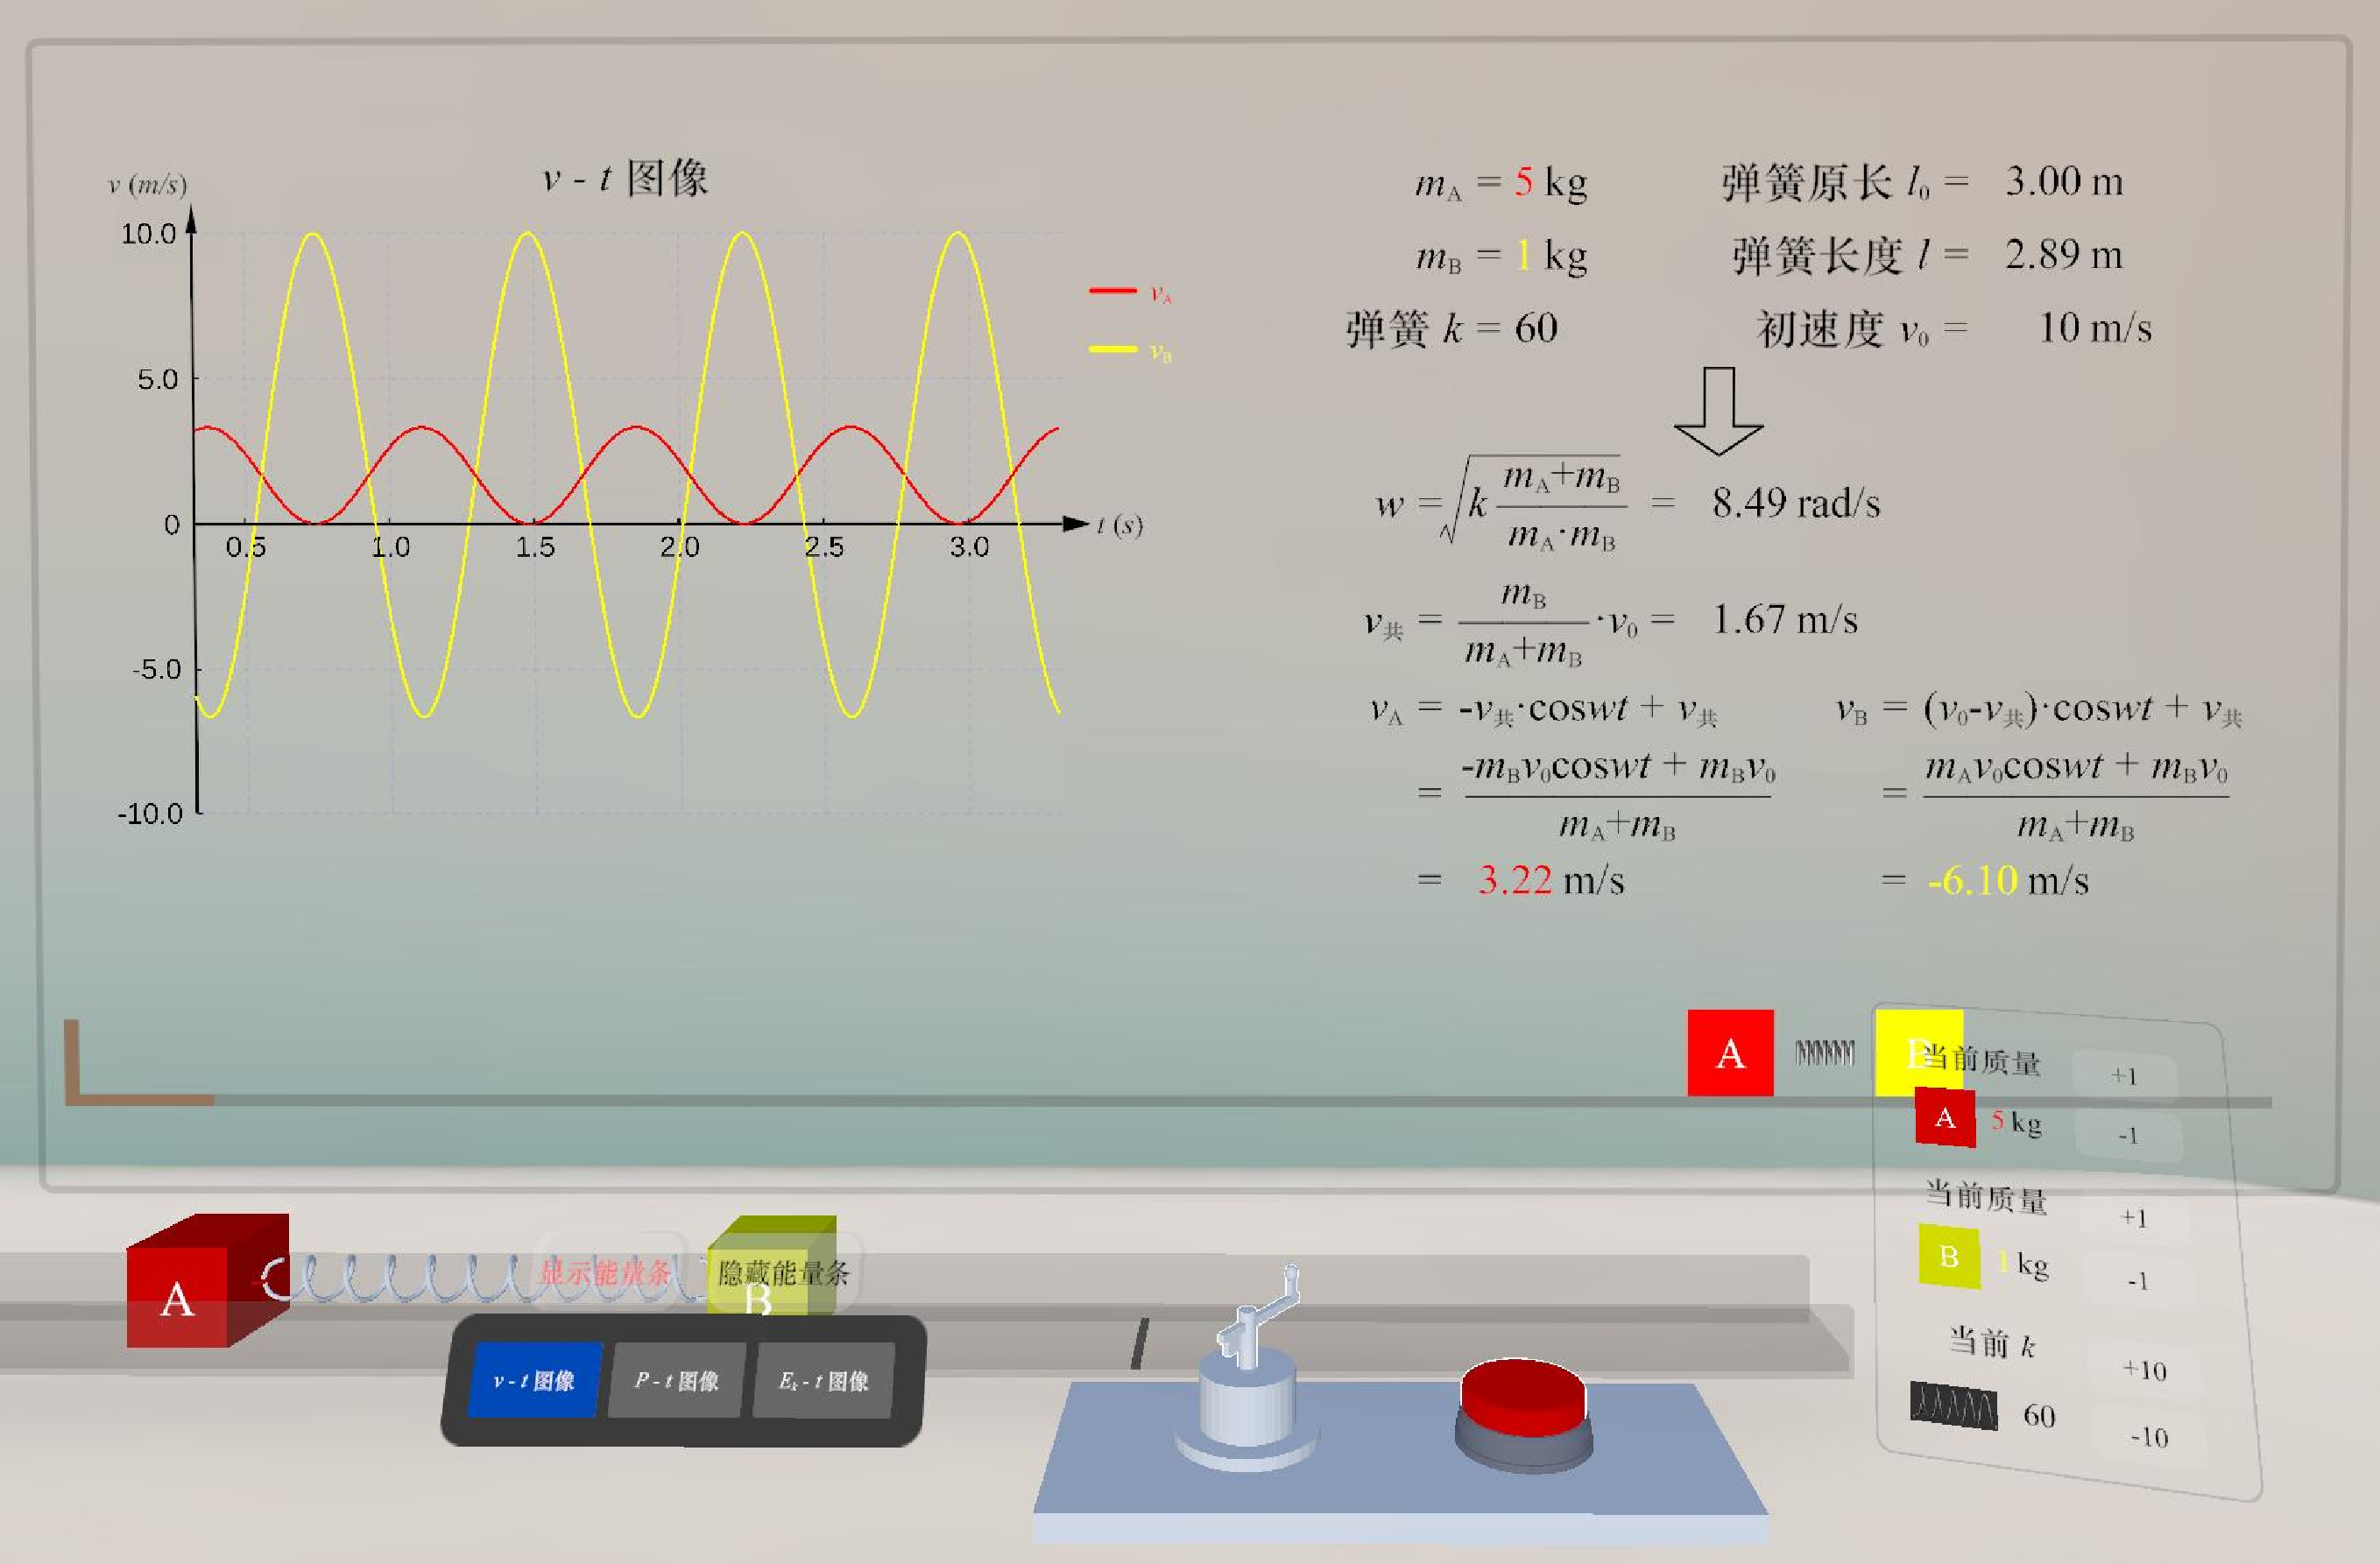
\includegraphics[width=1\textwidth]{image/experiment-scenario.pdf}
  \caption{Experimental scenario}
  \label{fig:experiment-scenario}
\end{figure*}

\section{Evaluation}
\subsection{Hypotheses}
Compare the two interaction methods of VRTI and GI. Based on previous related haptic studies, we make the following hypotheses:

\begin{itemize}[label=\(\bullet\)]
  \item \textbf{H1}: Adding haptic feedback to gesture interaction can enhance students' interest and participation in the experiment, and improve learning motivation. That is, VRTI is significantly higher than GI in terms of learning motivation.
  \item \textbf{H2}: Adding haptic feedback to gesture interaction can enhance students' sense of immersion and make them more deeply involved in the experiment process. That is, VRTI is significantly higher than GI in terms of sense of immersion.
\end{itemize}

\subsection{Methods}
For hypothesis \textbf{H1}, the Keller scale \cite{keller1983motivational} is used, which evaluates four dimensions based on the ARCS motivation model: attention, relevance, confidence, and satisfaction, to measure the learner's internal drive to participate in and complete learning tasks.

For hypothesis \textbf{H2}, the Schubert scale \cite{schubert2001experience} is used, focusing on the sense of presence in the virtual environment, and comprehensively evaluating students' sense of immersion and control through three dimensions: spatial presence, participation, and realism of the virtual environment.

All scales have been translated and localized to be suitable for the culture and educational background of this experiment, and their reliability has been verified through pre-testing (Cronbach's $\alpha$ > 0.8). In addition, after the participants completed the experiment, we randomly selected some participants for semi-structured interviews to collect their subjective experience and feedback on VRTI.

\subsection{Experiment}
The experiment uses Meta Quest 3 as the VR head-mounted display to provide visual information, and VRT as the interaction method to provide haptic feedback. The program interaction logic and visualization scenarios are implemented through Unity 2021.3.32f1c1. VRT uses gesture tracking technology to visualize the user's physical hand as a virtual hand for interaction, and realizes real-time data update and synchronization through sensing technology. Gesture tracking is implemented through Meta XR All-in-One SDK (v63). The system framework is shown in Figure \ref{fig:system-framework-flowchart}.

\begin{figure*}[t]
  \centering
  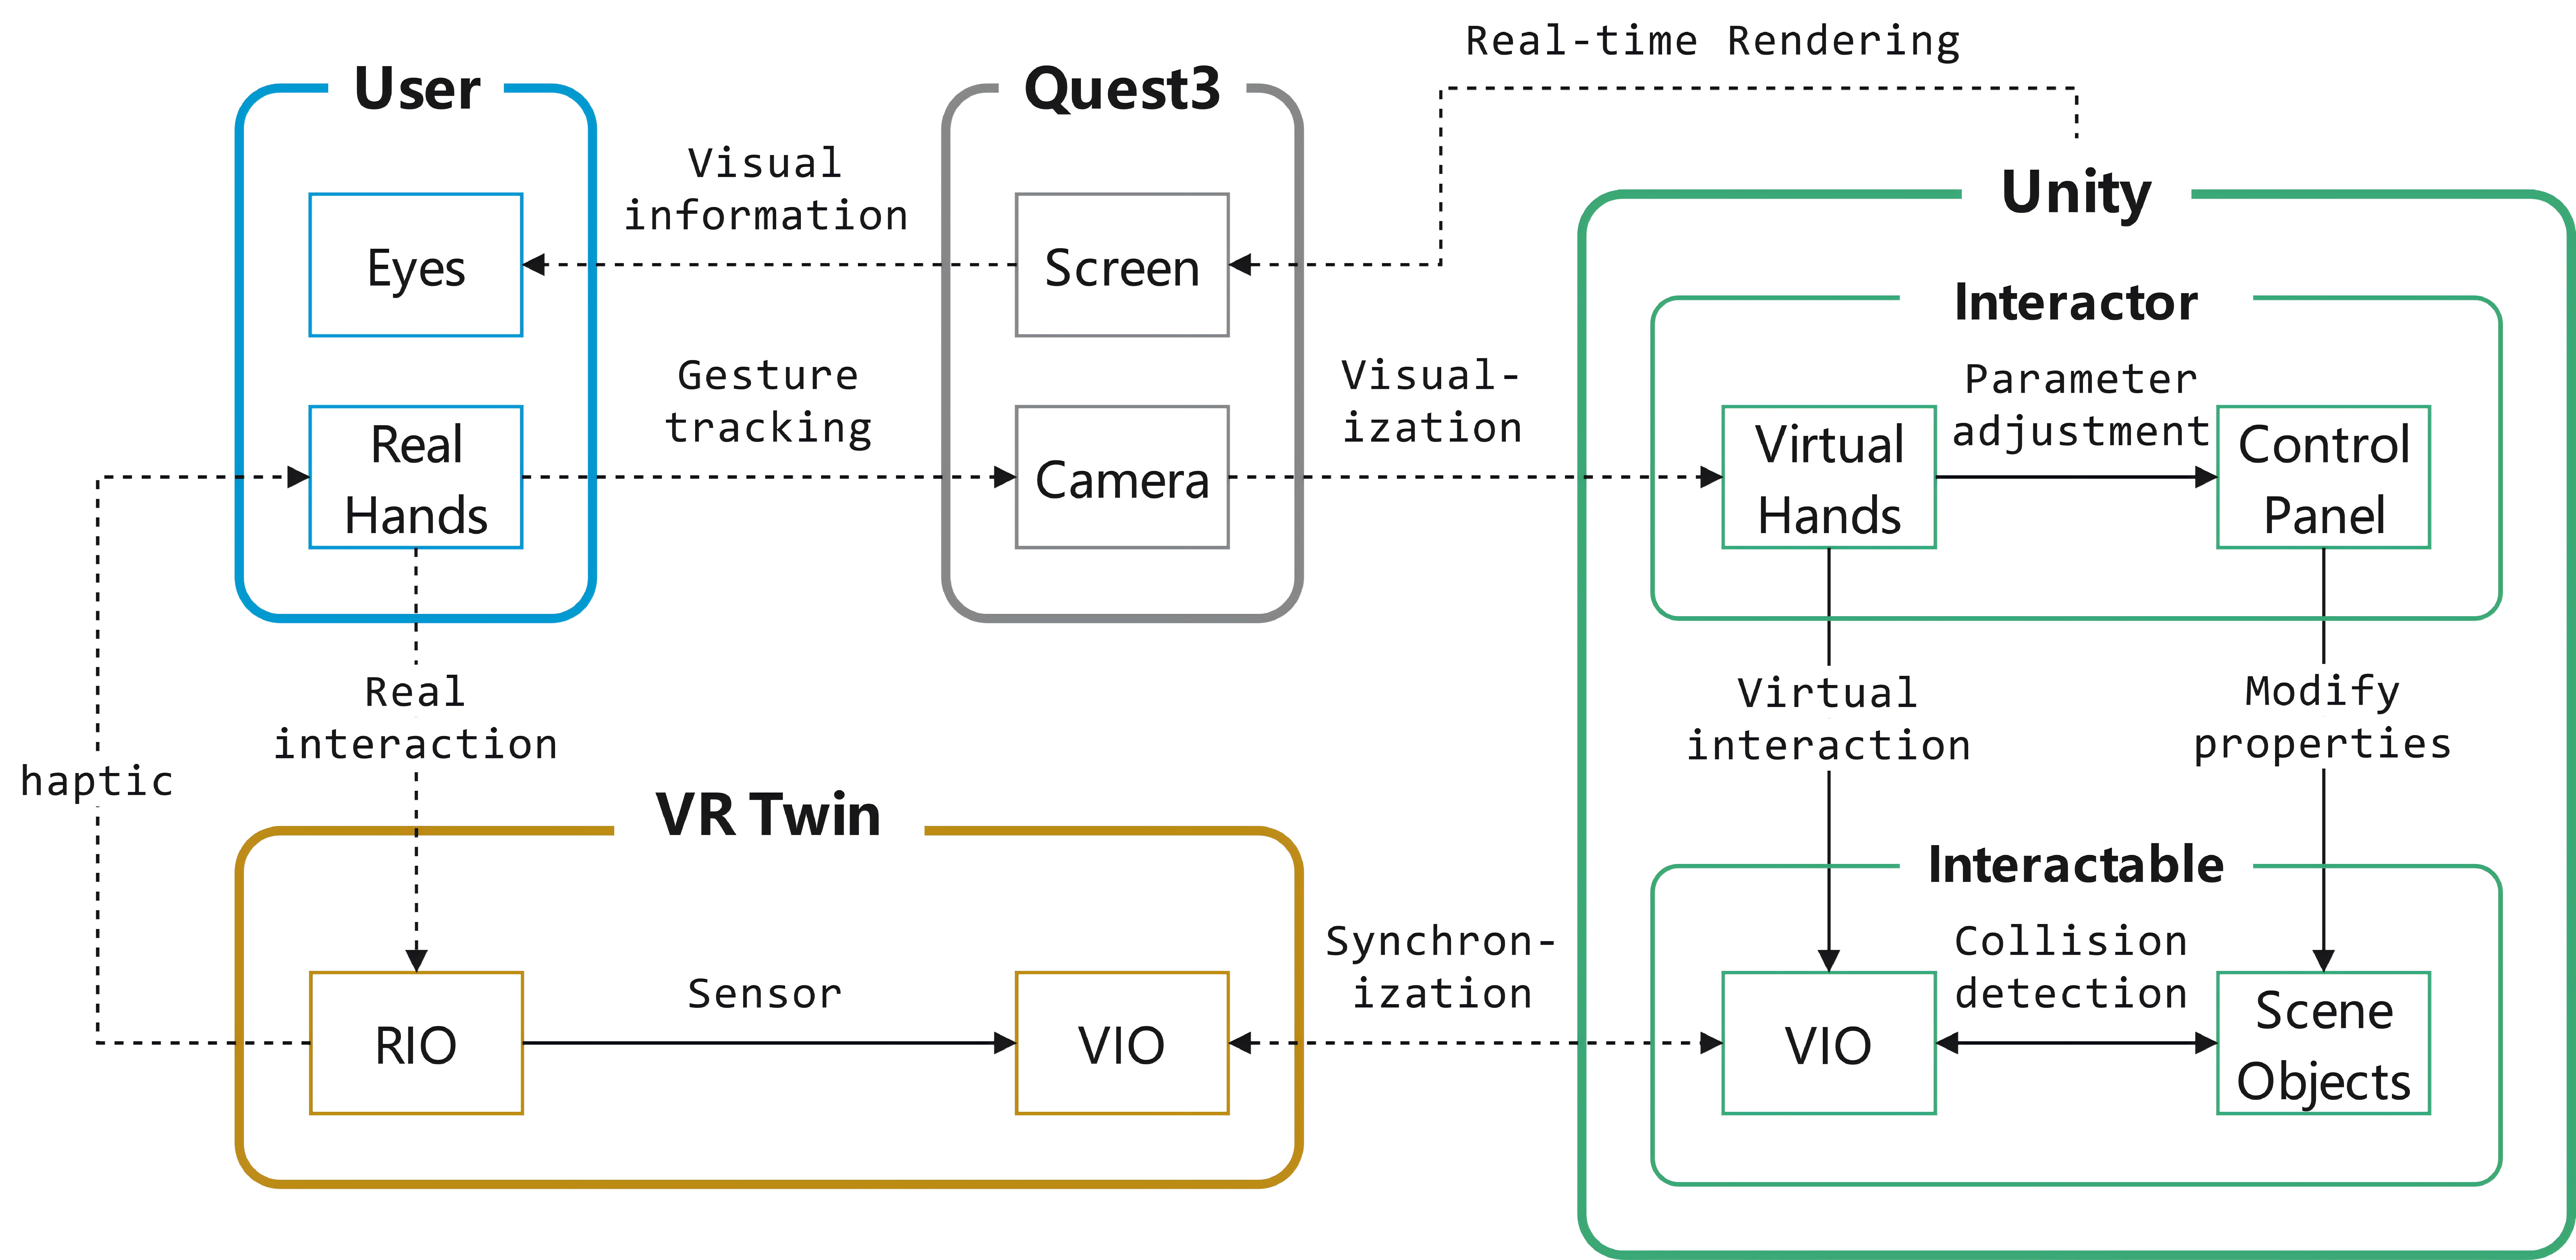
\includegraphics[width=1\textwidth]{image/system-framework-flowchart.pdf}
  \caption{System framework}
  \label{fig:system-framework-flowchart}
\end{figure*}

\subsection{Procedure}
\subsubsection{Participants}
64 high school students from a local XXX school were recruited to participate in the experiment. The age of the participants ranges from 16 to 18 years old. All participants have normal vision or corrected to normal vision. Participants were randomly divided into two groups, among which the GI group only relied on gestures to trigger the movement of virtual objects, without physical proxies and force feedback.

\begin{enumerate}[label={\arabic*)}]
  \item \texttt{Experimental Group} N=32, using VRTI interaction.
  \item \texttt{Control Group} N=32, using GI interaction.
\end{enumerate}

\subsubsection{Experimental Steps}
After entering the experiment, students first adjust the mass of blocks A and B and the spring stiffness coefficient through the physical parameter panel on the right. Secondly, make a grasping gesture to grab block B on the right, pull it to the right for a certain distance and release it, so that block B gains an initial velocity under the pull of the spring, and the system then performs periodic motion. The instantaneous velocity vector and resultant force vector are displayed above blocks A and B respectively. The subsystem is stationary at a certain time point. Rotate the knob clockwise to advance the system time; rotate the knob counterclockwise to rewind the system time. Finally, make a pressing gesture to press the button, and the system will continue to run from the current time point. When the system is in motion, pressing the button will restore the system to its initial state.

\subsubsection{Supervision and Guidance}
To ensure the validity of the results, all participants received unified experiment introduction and operation guidance before the experiment, and teaching assistants were assigned to supervise to ensure that each participant followed the experimental steps, as shown in Figure \ref{fig:experimental-procedure}. The process includes the following four steps:

\begin{enumerate}[label={\arabic*)}]
  \item \texttt{Experiment Introduction} Students watch an instructional video to familiarize themselves with the experimental operation process.
  \item \texttt{Calibration} Students perform hand calibration under the guidance of teaching assistants to align the user's hand with the virtual hand.
  \item \texttt{Experimental Operation} Students conduct experiments by group.
  \item \texttt{Post-test} Students independently complete a user experience questionnaire, including 10 items on learning motivation and 12 items on sense of immersion.
\end{enumerate}

\begin{figure}
  \begin{subfigure}{0.48\linewidth}
  \centering
  \includegraphics[width=\linewidth]{image/experimental-introduction.pdf}
  \caption{}
  \label{fig:experimental-introduction}
  \end{subfigure}
  \hfill
  \begin{subfigure}{0.48\linewidth}
  \centering
  \includegraphics[width=\linewidth]{image/experimental-operation.pdf}
  \caption{}
  \label{fig:experimental-operation}
  \end{subfigure}
  \caption{Experiment demonstration. (\subref{fig:experimental-introduction}) Experiment introduction, (\subref{fig:experimental-operation}) Experiment operation}
  \label{fig:experimental-procedure}
\end{figure}

\subsection{Result Analysis}
To verify hypotheses \textbf{H1} and \textbf{H2}, we used the Shapiro-Wilks test on the data of the experimental group and the control group. The results showed that neither group followed a normal distribution, so the Mann-Whitney U test was used to analyze the differences between groups. In the following data, a significance level of \(p \le 0.05\) () indicates a significant difference, \(p \le 0.01\) () indicates a highly significant difference, and \(p \le 0.001\) () indicates an extremely significant difference. The explanation of effect size refers to Cohen's criteria: |r|=0.1 is a small effect, 0.3 is a medium effect, and 0.5 is a large effect.

Figure \ref{fig:user-experience-result} compares the experimental results of the two groups in terms of learning motivation and sense of immersion. The solid dots above each group are sample points, and the kernel smoothing fitting curve describes their distribution. The Type I box plot below shows the 25\% (Q1), 50\% (Q2), and 75\% (Q3) quantiles. The experimental group showed a significant improvement in learning motivation (\(Z=-3.509,p<0.001,|r|=0.620\)) and sense of immersion (\(Z=-4.751,p<0.001,|r|=0.840\)), which is a large effect. Therefore, we have sufficient reason to accept hypotheses \textbf{H1} and \textbf{H2}. During the experiment, none of the participants reported any discomfort or motion sickness symptoms.

\begin{figure*}[t]
  \centering
  \includegraphics[width=0.75\textwidth]{image/user-experience-result.pdf}
  \caption{Comparison of results between VRTI group and GI group in terms of learning motivation and sense of immersion}
  \label{fig:user-experience-result}
\end{figure*}

Further analysis of learning motivation and sense of immersion found that the VRTI group was significantly better than the GI group in all 4 dimensions of learning motivation and 3 dimensions of sense of immersion, and the results are shown in Figure \ref{fig:three-user-experience-result}.

\begin{figure*}[t]
  \centering
  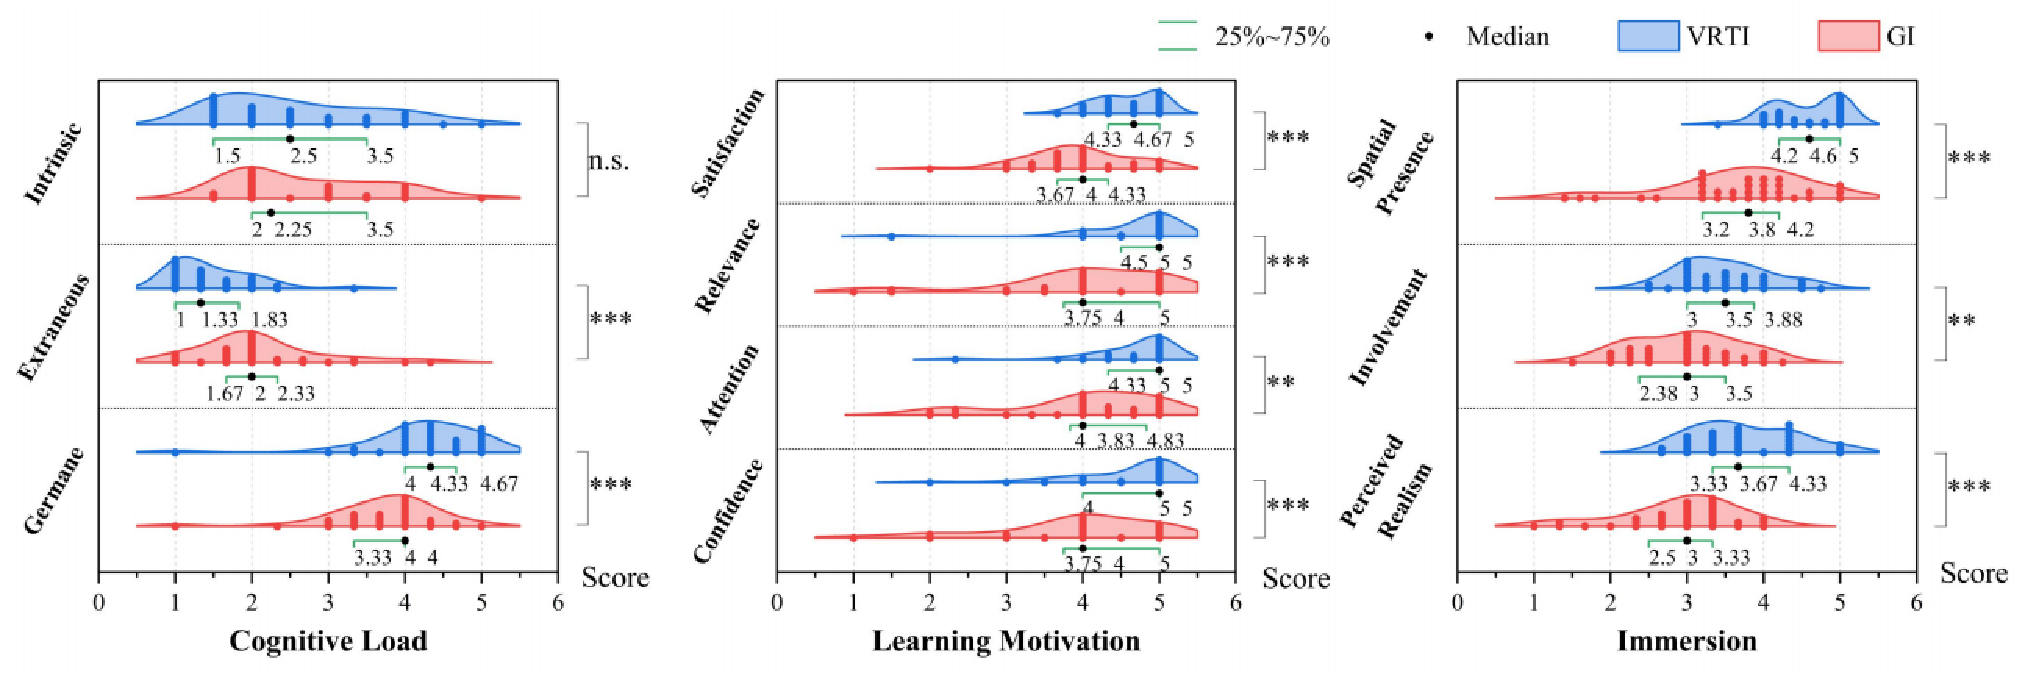
\includegraphics[width=\textwidth]{image/three-user-experience-result.pdf}
  \caption{Comparison of VRTI and GI in various user experience dimensions}
  \label{fig:three-user-experience-result}
\end{figure*}

\subsubsection{Learning Motivation}
In the attention dimension (\(Z=-3.382,p=0.001,|r|=0.598\)), the haptic feedback of VRTI can better attract students' attention and reduce distraction; in the relevance dimension (\(Z=-3.313,p=0.001,|r|=0.586\)), students in the VRTI group are more likely to connect virtual experiments with real knowledge, enhancing the practical significance of learning content; in the confidence dimension (\(Z=-3.001,p=0.003,|r|=0.531\)), the haptic feedback of VRTI helps students complete experimental tasks more confidently and reduces operational difficulty; in the satisfaction dimension (\(Z=-4.127,p<0.001,|r|=0.730\)), students in the VRTI group are more recognized and satisfied with the overall learning experience.

\subsubsection{Sense of Immersion}
In the spatial presence dimension (\(Z=-4.021,p<0.001,|r|=0.712\)), the synchronous haptic feedback of VRTI makes it easier for students to perceive the spatial relationship between themselves and the virtual environment, enhancing the "being there" experience; in the participation dimension (\(Z=-3.765,p<0.001,|r|=0.667\)), students in the VRTI group showed higher active participation and continuous engagement in the experiment process, and the interaction process was more attractive; in the virtual environment realism dimension (\(Z=-4.512,p<0.001,|r|=0.800\)), the dynamic haptic feedback of VRTI significantly improved the realism and credibility of virtual experiments.

\subsubsection {Semi-structured Interviews}
Combined with user interviews, some students reported that the real haptic experience of VRTI made them "as if doing real experiments", more willing to immerse themselves and focus on experimental tasks, and actively explore and operate repeatedly. Compared with the traditional GI group, students in the VRTI group showed stronger initiative and exploration desire during the experiment, willing to try different parameter settings and interaction methods, and the overall immersive experience was better. These results further verify the effectiveness and application potential of VRTI in improving learning motivation and sense of immersion.

\section{Discussion and Future Work}
\subsubsection{Promoting Automatic Calibration}
Each deployment of the experiment requires manual calibration to align the initial position of the user's hand with the virtual hand, which does not support independent experiments by users and is cumbersome to operate. Future research will explore automatic calibration methods, using gesture tracking technology to detect the user's hand position and posture in real-time, and automatically adjust the alignment between the virtual hand and physical interaction objects. Machine learning algorithms will be used to analyze user hand movement patterns to achieve more intelligent initial alignment and reduce user operation burden.

\subsubsection {Prop Design}
During the experiment interviews, some users suggested optimizing the support structure of the device to reduce operational fatigue: "If a support frame can be designed so that the arm doesn't have to be suspended all the time, it will be easier to operate." Future research will explore more ergonomic prop designs, optimize the support structure and handle shape, and improve user operation comfort and experience. At the same time, consider implementing user personalized customized props to meet the hand size and operating habits of different users.

\subsubsection{Prop Durability}
In addition, users also mentioned the need to improve the durability of the device: "The tactile feedback of the device decreased after multiple uses, and it is hoped that this can be improved in the future." Future research will explore more durable materials to improve the durability of the device's haptic feedback and ensure stable haptic experience during long-term use. At the same time, consider introducing replaceable haptic feedback modules to facilitate users to adjust and maintain the device as needed.

\section{Conclusion}
This paper proposes the Virtual-Reality Twin Interaction (VRTI) framework, which improves the gesture interaction experience in immersive learning environments through dynamic passive haptic feedback and haptic retargeting technology. A VRT prototype supporting three basic operations: grasping, pressing, and pinching is developed based on VRTI and applied to an immersive learning environment. User studies show that VRTI not only enhances learners' learning motivation but also improves their sense of immersion and participation, and interview results further verify its effectiveness and application potential. Future work will focus on automatic calibration, optimization of prop design, and improvement of device durability to promote the wide application of VRTI in education and other fields.

\begin{credits}
\subsubsection{\ackname}
This research was supported by the National Natural Science Foundation of XXX.
% China XXX
% (Grant No. 62377004)

\subsubsection{\discintname}
The authors declare no conflict of interest.
\end{credits}

\bibliography{VRTI-bib}

\end{document}

